\chapter[Resultados y Análisis]{Resultados y Análisis}
\label{chap:resultados}

\insertminitoc
\parindent0pt


\section{Presentación de los resultados}

Este capítulo presenta la evaluación del sistema de reconocimiento del \Acrshort{lesho}. Se organiza en seis partes: el desempeño del modelo del alfabeto dactilológico (Modelo A), el desempeño del modelo de señas dinámicas (Modelo B), la comparación entre ambos, la evaluación del sistema ejecutándose sobre el dispositivo, los instrumentos diseñados para medir la usabilidad con las personas usuarias, y una discusión integral de los hallazgos.

La evaluación de los modelos se realizó con una división estratificada por clase y agrupada por toma: ninguna toma de captura cruzó de la partición de entrenamiento a la de prueba, y todas las clases con datos aparecen en las particiones. Esta decisión evita la fuga de datos que produce la división aleatoria por ventana, en la que fragmentos casi idénticos de una misma grabación caen a la vez en entrenamiento y prueba e inflan la exactitud de forma ficticia. En consecuencia, las cifras que se reportan miden el desempeño sobre tomas que el modelo no vio nunca. Todas las figuras de este capítulo son de elaboración propia.


\section{Desempeño del Modelo A (alfabeto dactilológico)}

El Modelo A clasifica una ventana temporal corta de fotogramas de landmarks en las 33 clases con que fue entrenado: las 30 letras del alfabeto dactilológico, la clase de reposo y las dos señas de control que se evaluaron durante el desarrollo y que la versión final del sistema no utiliza. Estas dos últimas aparecen en las figuras de este capítulo con las etiquetas INICIO y FIN, que son los nombres con que se grabaron. La Tabla~\ref{tab:metricas-a} resume sus métricas globales sobre la partición de prueba.

\begin{table}[h!]
\centering
\begin{tabular}{lc}
\hline
\textbf{Métrica} & \textbf{Valor} \\
\hline
Exactitud global & 99.54\% \\
Puntaje F1 (macro) & 0.995 \\
Número de clases & 33 \\
Muestras de prueba & 4,364 \\
Parámetros del modelo & 24,929 \\
Tamaño en \Acrshort{tflite} & 33.9 KB \\
\hline
\end{tabular}
\caption{Métricas globales del Modelo A sobre la partición de prueba.}
\label{tab:metricas-a}
\end{table}

La exactitud global de \textbf{99.54\%} y el puntaje F1 macro de \textbf{0.995} indican que el modelo separa con solidez las clases del alfabeto. El valor F1 macro, que promedia el desempeño de todas las clases por igual sin importar cuántas muestras tenga cada una, confirma que el resultado no depende de unas pocas clases mayoritarias.

La Figura~\ref{fig:curvas-a} muestra la evolución de la exactitud y de la pérdida durante el entrenamiento, tanto en el conjunto de entrenamiento como en el de validación.

\begin{figure}[htbp]
    \centering
    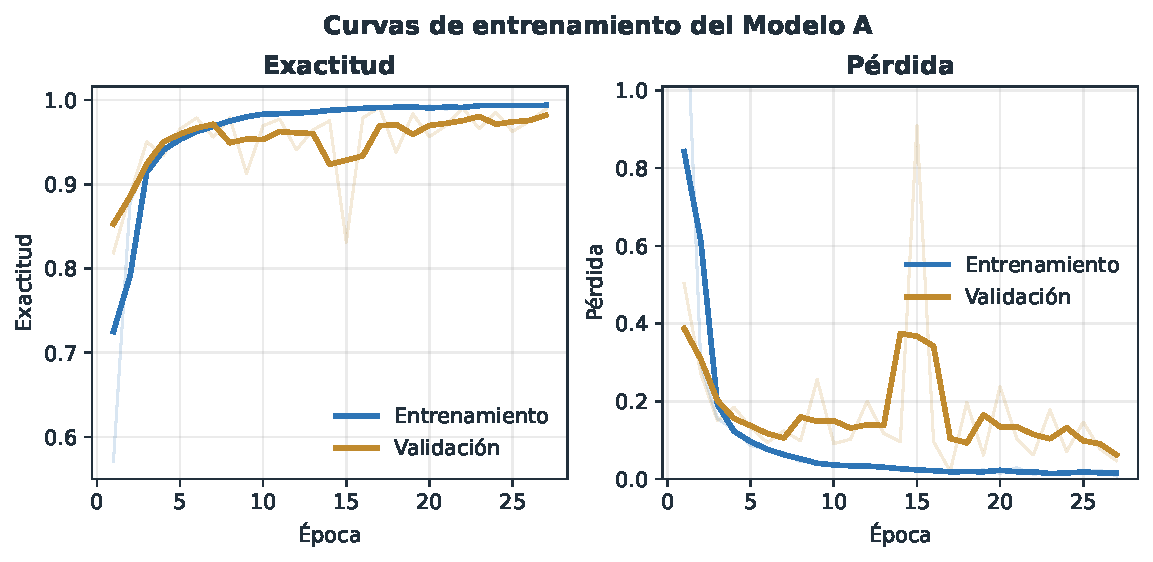
\includegraphics[width=1\linewidth]{Figures/Resultados/curvas_entrenamiento_a.pdf}
    \caption[Curvas de entrenamiento del Modelo A]{Curvas de entrenamiento del Modelo A: exactitud y pérdida por época. La línea marcada es el promedio móvil y la línea tenue el valor de cada época. Fuente: Elaboración propia.}
    \label{fig:curvas-a}
\end{figure}

Las curvas de la Figura~\ref{fig:curvas-a} muestran una convergencia estable. La pérdida de validación desciende junto con la de entrenamiento y no vuelve a subir de forma sostenida, lo que indica que el mecanismo de parada temprana detuvo el ajuste antes de que apareciera un sobreajuste marcado. La cercanía entre las curvas de entrenamiento y de validación es una señal de que el modelo generaliza dentro del corpus disponible.

Para observar el detalle por clase, la Figura~\ref{fig:confusion-a} presenta la matriz de confusión y la Figura~\ref{fig:f1-a} el puntaje F1 de cada clase.

\begin{figure}[htbp]
    \centering
    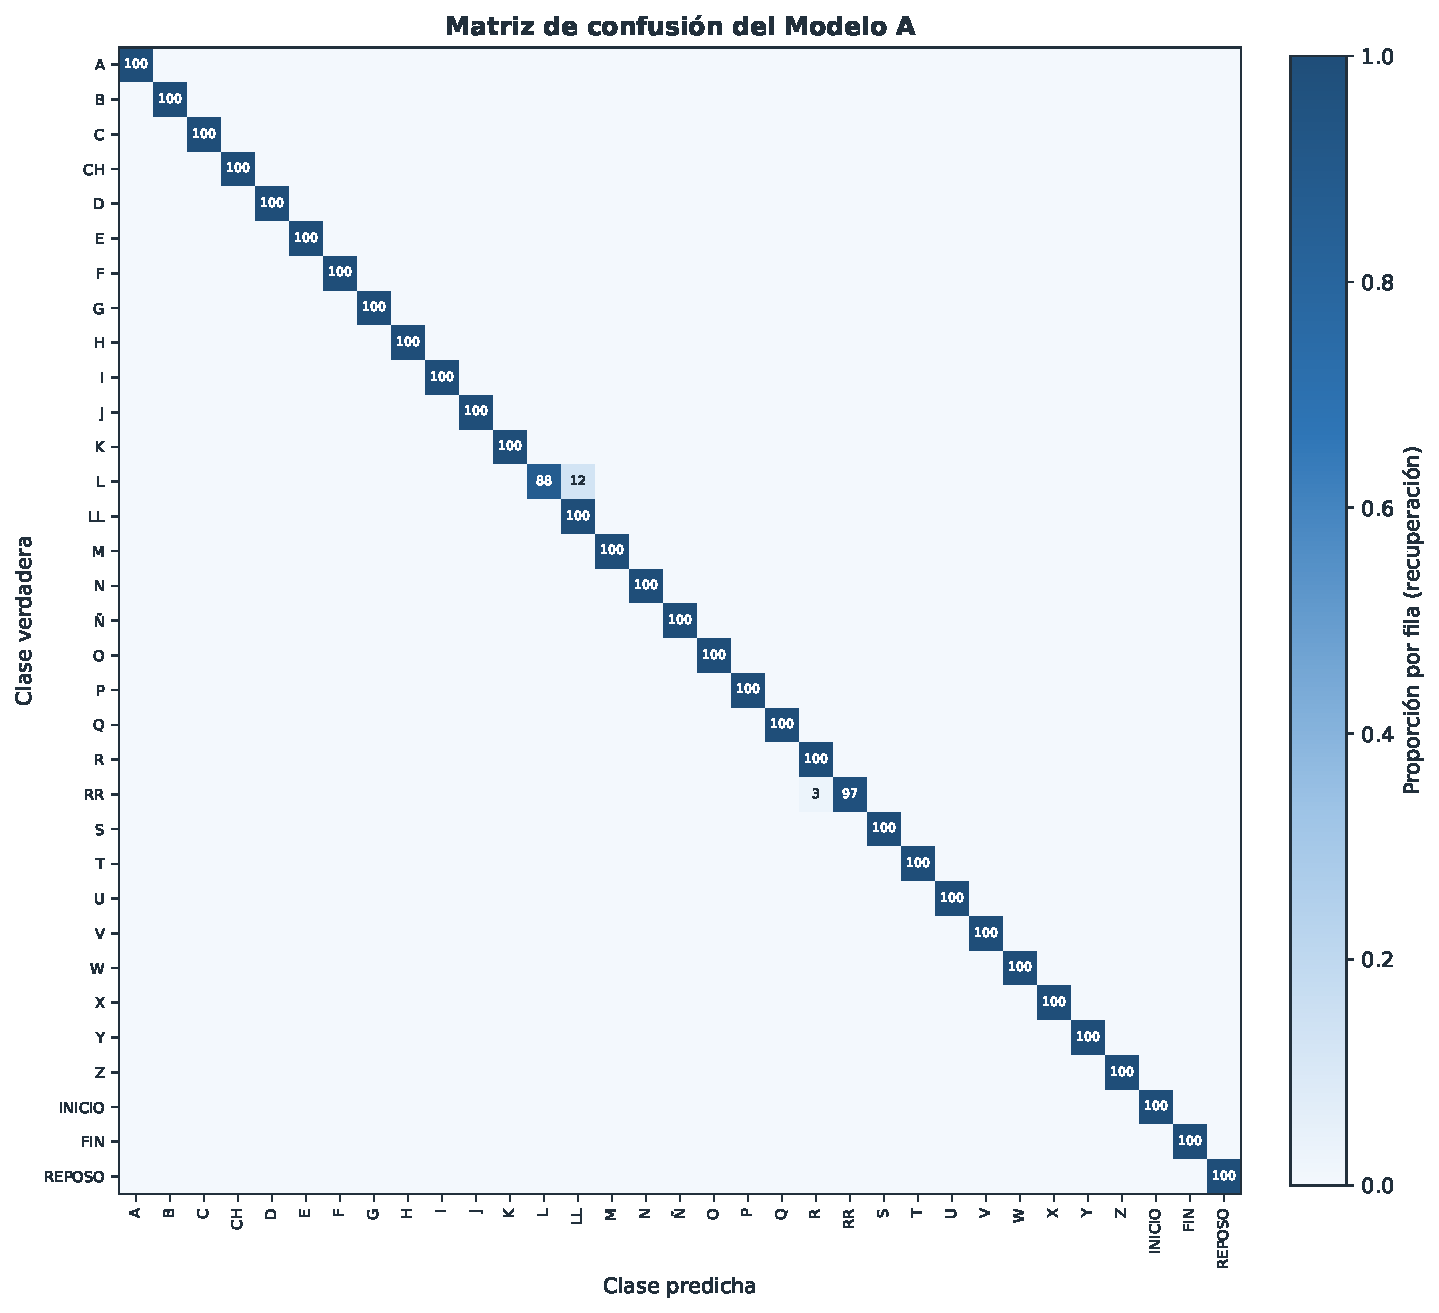
\includegraphics[width=0.9\linewidth]{Figures/Resultados/matriz_confusion_a.pdf}
    \caption[Matriz de confusión del Modelo A]{Matriz de confusión del Modelo A, normalizada por fila. Fuente: Elaboración propia.}
    \label{fig:confusion-a}
\end{figure}

En la matriz de confusión de la Figura~\ref{fig:confusion-a}, la diagonal concentra casi toda la masa, lo que refleja la alta exactitud. Las confusiones que aparecen fuera de la diagonal son coherentes con la naturaleza del alfabeto dactilológico: se dan entre letras de forma de mano parecida. Las cinco letras que se ejecutan con movimiento, que son la J, la Ñ, la Z, la LL y la RR, son las más sensibles, porque su reconocimiento depende de la trayectoria completa y esa trayectoria varía más entre personas que la forma de una pose fija.

\begin{figure}[htbp]
    \centering
    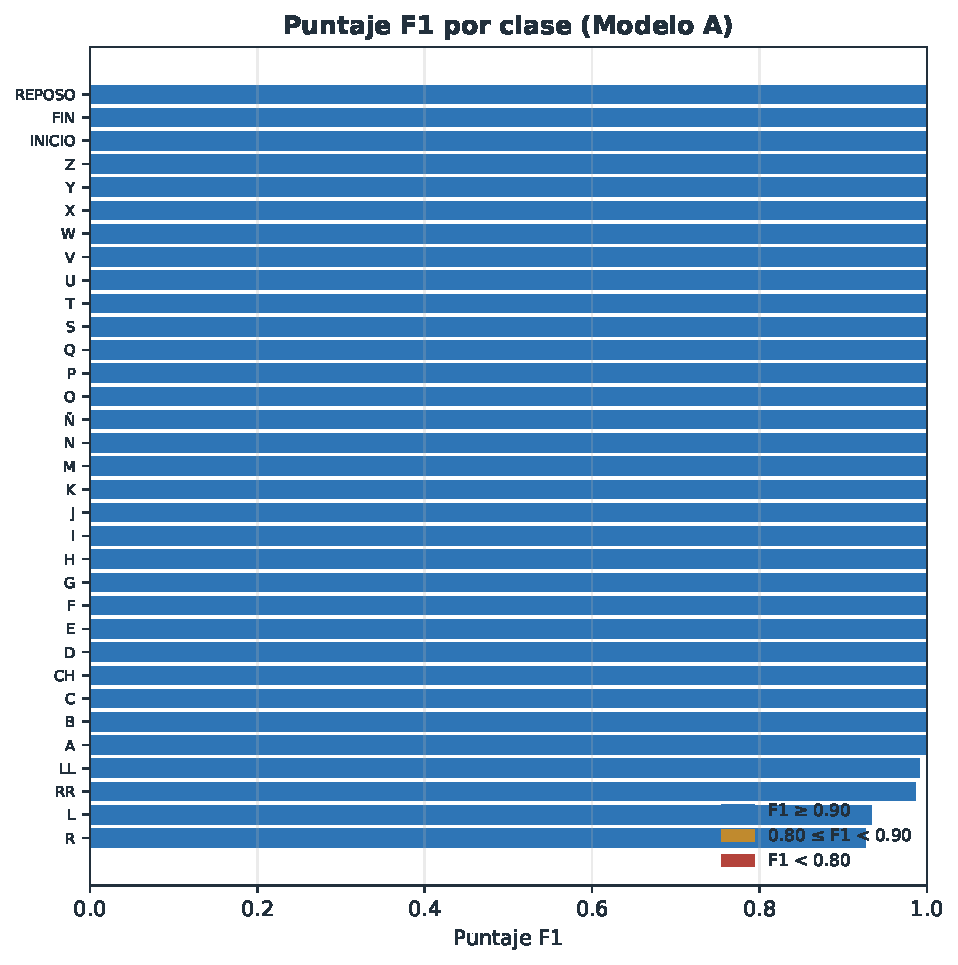
\includegraphics[width=0.68\linewidth]{Figures/Resultados/f1_por_clase_a.pdf}
    \caption[Puntaje F1 por clase del Modelo A]{Puntaje F1 por clase del Modelo A, ordenado de menor a mayor. Fuente: Elaboración propia.}
    \label{fig:f1-a}
\end{figure}

La Figura~\ref{fig:f1-a} confirma que la gran mayoría de las clases supera un F1 de 0.90. Las pocas clases con un valor menor corresponden a las letras con movimiento y a algunas letras estáticas de forma similar. Este comportamiento es el esperado y se explica por la variabilidad natural del gesto, no por un defecto del modelo.


\section{Desempeño del Modelo B (señas dinámicas)}

El Modelo B es una red \acrfull{lstm} ligera que clasifica una secuencia completa de landmarks en las 50 señas dinámicas del vocabulario. A diferencia del Modelo A, cada fotograma incorpora, además de la configuración de las manos, la ubicación de estas respecto al cuerpo, obtenida con el marco de referencia de los hombros y de las anclas de la cara. La Tabla~\ref{tab:metricas-b} resume sus métricas globales sobre la partición de prueba.

\begin{table}[h!]
\centering
\begin{tabular}{lc}
\hline
\textbf{Métrica} & \textbf{Valor} \\
\hline
Exactitud global & 98.80\% \\
Puntaje F1 (macro) & 0.988 \\
Número de señas & 50 \\
Muestras de prueba & 834 \\
Parámetros del modelo & 61,122 \\
Tamaño en \Acrshort{tflite} & 78.1 KB \\
\hline
\end{tabular}
\caption{Métricas globales del Modelo B sobre la partición de prueba.}
\label{tab:metricas-b}
\end{table}

La exactitud global de \textbf{98.80\%} y el F1 macro de \textbf{0.988} muestran que el modelo distingue con claridad las señas del vocabulario. La Figura~\ref{fig:curvas-b} presenta las curvas de entrenamiento.

\begin{figure}[htbp]
    \centering
    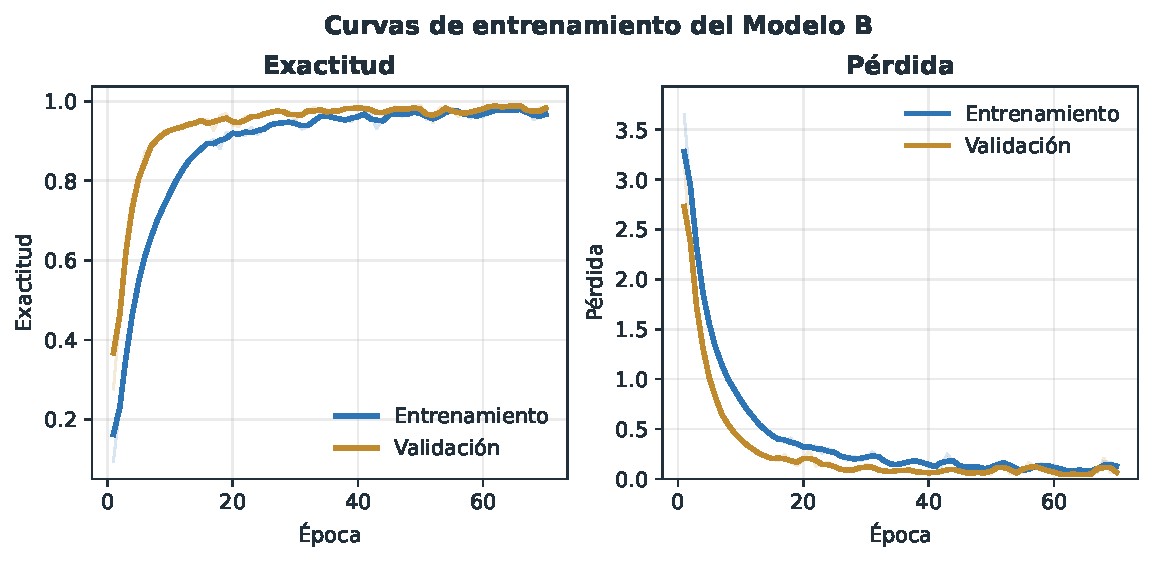
\includegraphics[width=1\linewidth]{Figures/Resultados/curvas_entrenamiento_b.pdf}
    \caption[Curvas de entrenamiento del Modelo B]{Curvas de entrenamiento del Modelo B: exactitud y pérdida por época. La línea marcada es el promedio móvil y la línea tenue el valor de cada época. Fuente: Elaboración propia.}
    \label{fig:curvas-b}
\end{figure}

Como se aprecia en la Figura~\ref{fig:curvas-b}, la validación alcanza valores altos y se mantiene cercana a la curva de entrenamiento, lo que indica que la arquitectura aprende la tarea sin un sobreajuste marcado. La parada temprana detiene el entrenamiento cuando la pérdida de validación deja de mejorar.

La Figura~\ref{fig:confusion-b} presenta la matriz de confusión de las 50 señas.

\begin{figure}[htbp]
    \centering
    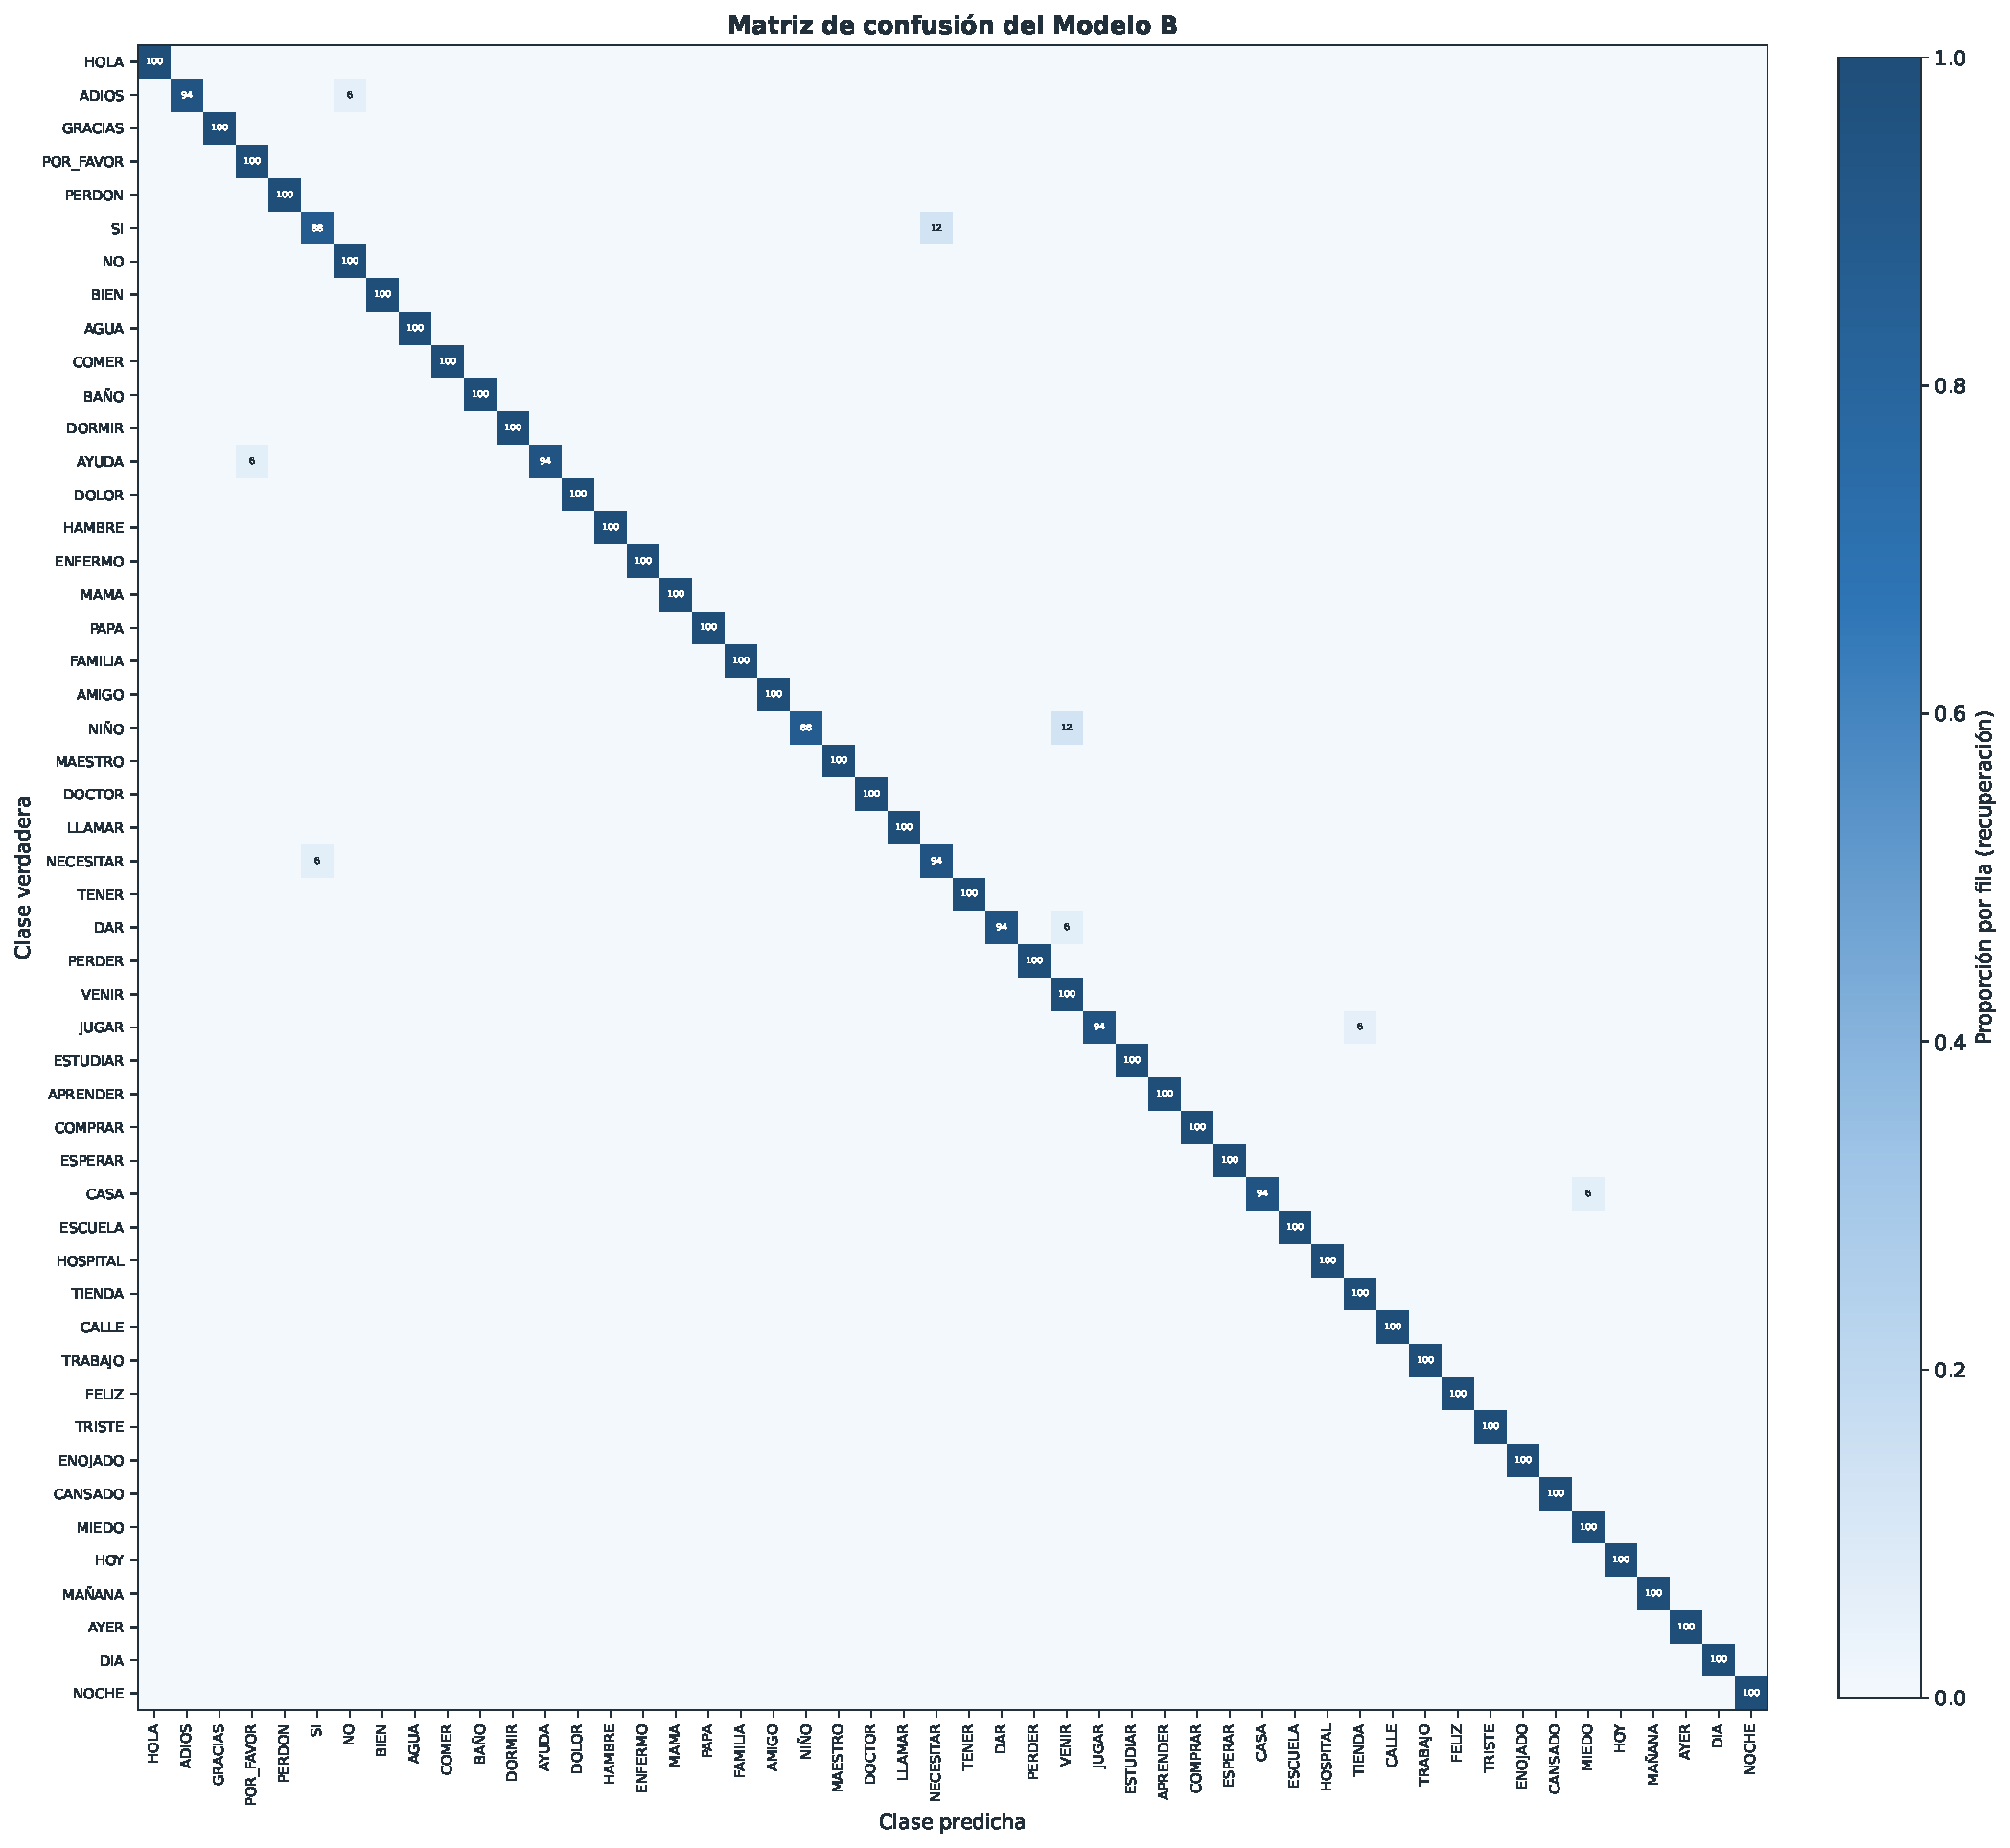
\includegraphics[width=1\linewidth]{Figures/Resultados/matriz_confusion_b.pdf}
    \caption[Matriz de confusión del Modelo B]{Matriz de confusión del Modelo B, normalizada por fila, sobre las 50 señas dinámicas. Fuente: Elaboración propia.}
    \label{fig:confusion-b}
\end{figure}

En la Figura~\ref{fig:confusion-b} la diagonal vuelve a concentrar la masa de aciertos. Las pocas confusiones que aparecen son leves y se dan entre señas que comparten el lugar de articulación y se distinguen por matices de forma o de movimiento de la mano. Este patrón valida una decisión central del diseño: incorporar la ubicación de la mano en el cuerpo, y en particular la posición de la punta del índice, fue lo que permitió separar señas que se hacen en zonas distintas de la cara, como HOLA en la frente y AGUA en la boca. Sin ese rasgo, ambas señas colapsaban en una sola.

La Figura~\ref{fig:f1-b} muestra el puntaje F1 por seña y la Figura~\ref{fig:radar-b} agrupa ese desempeño por categoría semántica.

\begin{figure}[htbp]
    \centering
    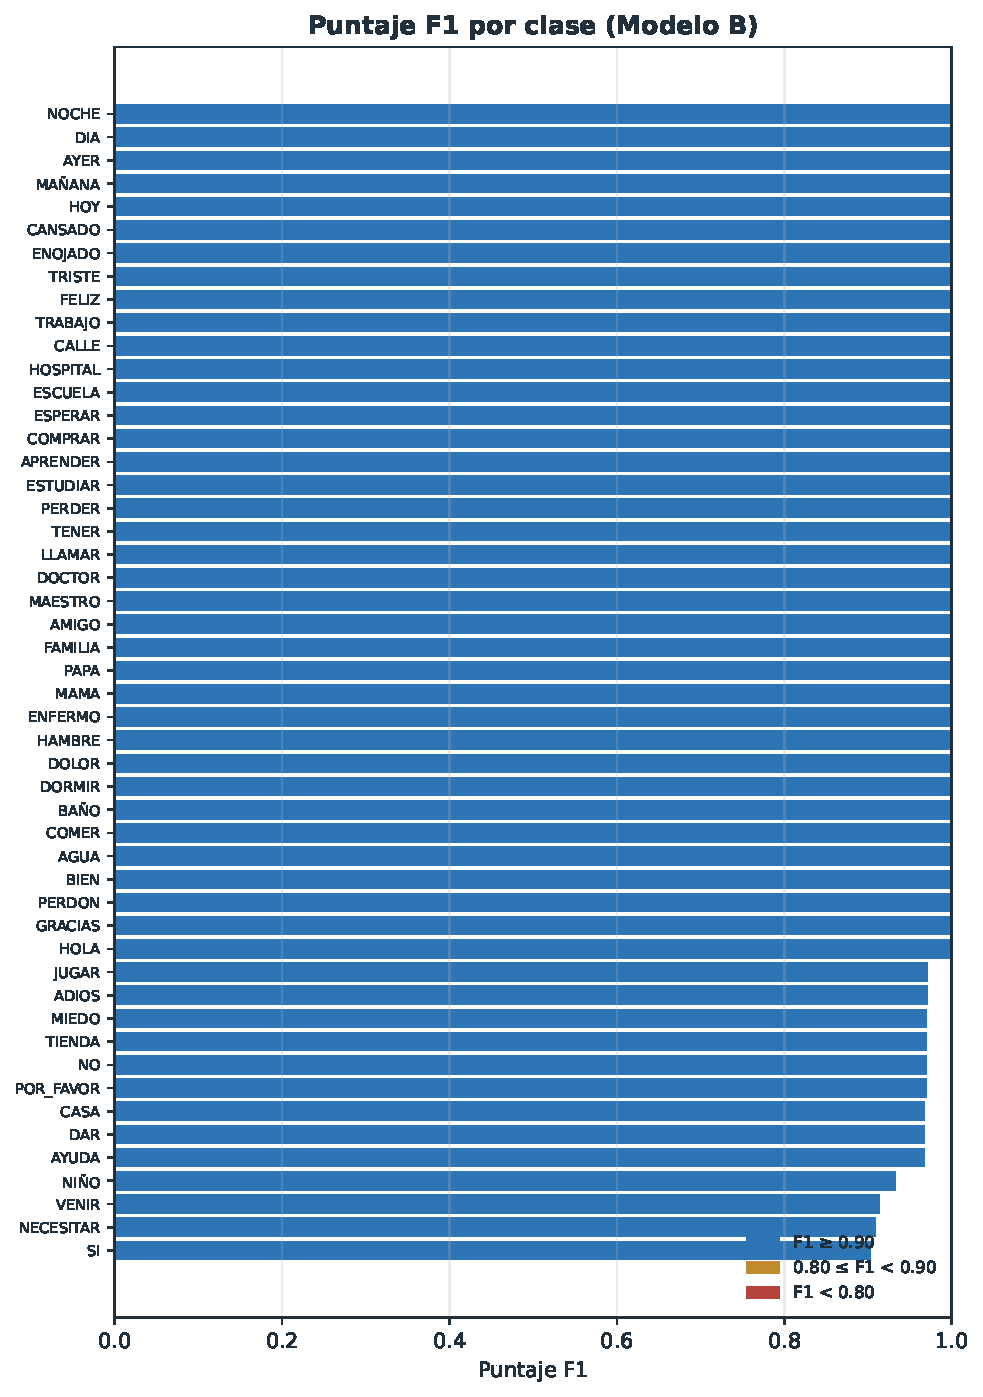
\includegraphics[width=0.68\linewidth]{Figures/Resultados/f1_por_clase_b.pdf}
    \caption[Puntaje F1 por seña del Modelo B]{Puntaje F1 por seña del Modelo B, ordenado de menor a mayor. Fuente: Elaboración propia.}
    \label{fig:f1-b}
\end{figure}

\begin{figure}[htbp]
    \centering
    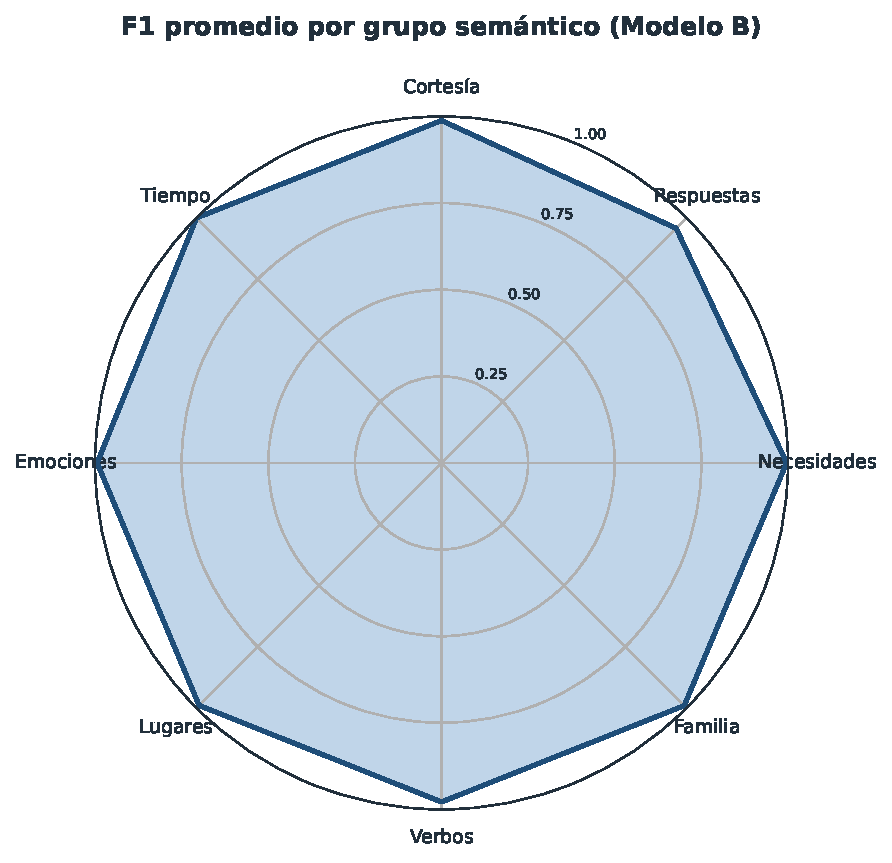
\includegraphics[width=0.62\linewidth]{Figures/Resultados/radar_grupos_b.pdf}
    \caption[F1 promedio por grupo semántico del Modelo B]{Puntaje F1 promedio por grupo semántico de señas del Modelo B. Fuente: Elaboración propia.}
    \label{fig:radar-b}
\end{figure}

El gráfico de araña de la Figura~\ref{fig:radar-b} resume el desempeño en las ocho categorías del vocabulario: cortesía, respuestas, necesidades, familia, verbos, lugares, emociones y tiempo. El polígono se acerca al borde exterior en todas las categorías, lo que indica un desempeño alto y parejo entre grupos. Las categorías con mayor variedad de señas, como verbos y necesidades, son las candidatas naturales a vigilar cuando el corpus siga creciendo.


\section{Comparación de los dos modelos}

Los dos modelos resuelven problemas distintos, pero conviene compararlos para justificar sus elecciones de diseño. La Figura~\ref{fig:radar-comparacion} los contrasta en cinco dimensiones y la Tabla~\ref{tab:arquitecturas} detalla sus arquitecturas.

\begin{figure}[htbp]
    \centering
    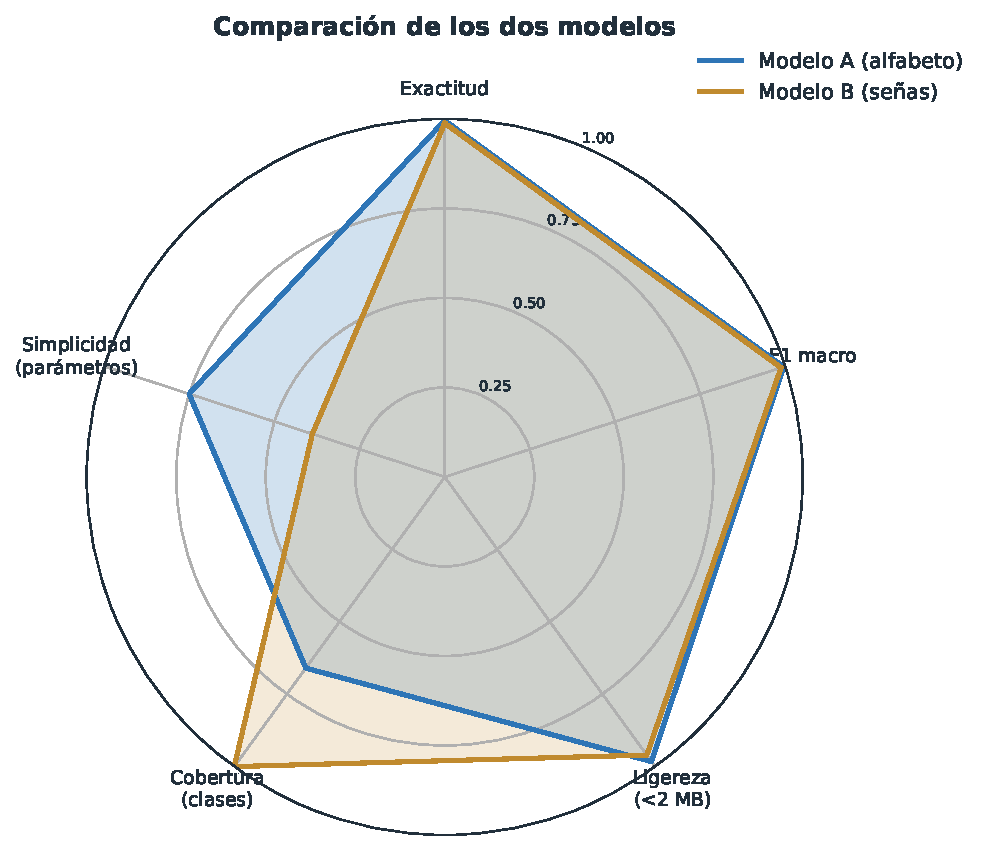
\includegraphics[width=0.62\linewidth]{Figures/Resultados/radar_comparacion.pdf}
    \caption[Comparación de los dos modelos]{Comparación del Modelo A y el Modelo B en exactitud, F1 macro, ligereza, cobertura y simplicidad. Fuente: Elaboración propia.}
    \label{fig:radar-comparacion}
\end{figure}

La Figura~\ref{fig:radar-comparacion} muestra que ambos modelos son livianos y precisos. El Modelo A resulta más simple, con menos parámetros, porque su tarea es clasificar una ventana corta con una red convolucional. El Modelo B tiene más parámetros y cubre más clases, ya que debe modelar secuencias completas con memoria temporal. Ambos se mantienen muy por debajo del límite de tamaño fijado para la ejecución en el teléfono.

\begin{table}[h!]
\centering
\resizebox{\textwidth}{!}{
\begin{tabular}{lcc}
\hline
\textbf{Característica} & \textbf{Modelo A (alfabeto)} & \textbf{Modelo B (señas)} \\
\hline
Tipo de red & Convolucional 1D & \Acrshort{lstm} \\
Entrada & Ventana de 20 fotogramas $\times$ 126 & Secuencia de 40 fotogramas $\times$ 152 \\
Clases de salida & 33 & 50 \\
Parámetros & 24,929 & 61,122 \\
Tamaño en \Acrshort{tflite} & 33.9 KB & 78.1 KB \\
Configuración de la mano & Una mano, espacio neutro & Dos manos con ubicación en el cuerpo \\
\hline
\end{tabular}}
\caption{Comparación de las arquitecturas de los dos modelos.}
\label{tab:arquitecturas}
\end{table}

La Tabla~\ref{tab:arquitecturas} sintetiza las diferencias. La elección de una red convolucional para el alfabeto y de una \Acrshort{lstm} para las señas responde al tipo de dato: una ventana corta para el primero y una secuencia larga con dependencia temporal para el segundo.


\section{Evaluación del sistema en el dispositivo}

Más allá de la exactitud, el sistema debe funcionar de forma completa en el teléfono, sin conexión a internet. Esta sección evalúa su costo de ejecución. La Figura~\ref{fig:velas-latencia} presenta la distribución de la latencia de inferencia de cada modelo.

\begin{figure}[htbp]
    \centering
    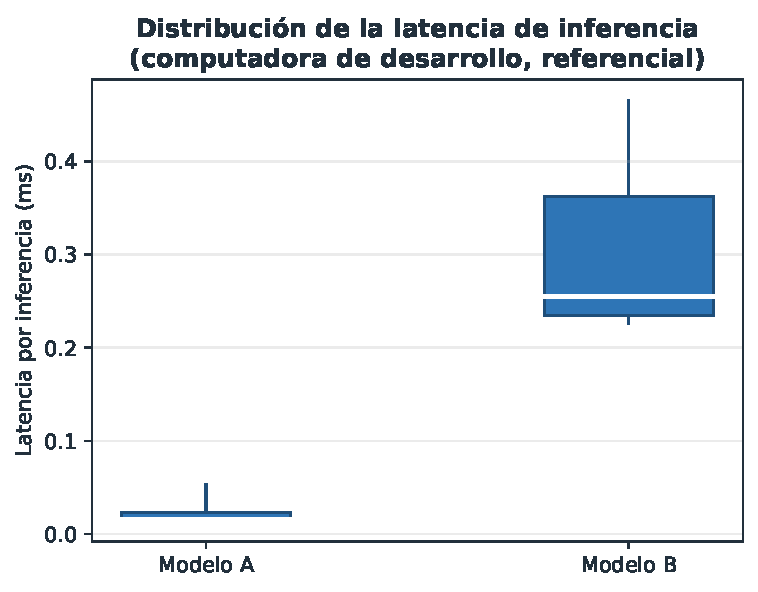
\includegraphics[width=0.55\linewidth]{Figures/Resultados/velas_latencia.pdf}
    \caption[Distribución de la latencia de inferencia]{Distribución de la latencia de inferencia por modelo, medida en la computadora de desarrollo como referencia. Fuente: Elaboración propia.}
    \label{fig:velas-latencia}
\end{figure}

El gráfico de velas de la Figura~\ref{fig:velas-latencia} representa, para cada modelo, la mediana, el rango entre el primer y el tercer cuartil y los valores mínimo y máximo de la latencia por inferencia. La inferencia de ambos modelos es muy rápida, del orden de milisegundos, lo que confirma que el clasificador no es el cuello de botella del sistema.

El costo real en el teléfono está dominado por la extracción de landmarks con MediaPipe, no por la inferencia de los modelos. Sobre el dispositivo de gama baja utilizado en las pruebas, un Samsung Galaxy A13, la aplicación procesa alrededor de 5 \Acrshort{fps} durante las señas dinámicas, que ejecutan la detección de las dos manos y del cuerpo en cada fotograma. El deletreo del alfabeto, que utiliza una sola mano y no ejecuta MediaPipe Pose, corre con mayor holgura. Esta diferencia explica que el reconocimiento del alfabeto se sienta más ágil que el de las señas dinámicas, y sustenta la recomendación de uso de sostener la posición inicial de la seña durante la captura.

La Figura~\ref{fig:recursos} resume el costo de recursos medido directamente sobre el dispositivo mientras la aplicación reconocía una seña dinámica.

\begin{figure}[htbp]
    \centering
    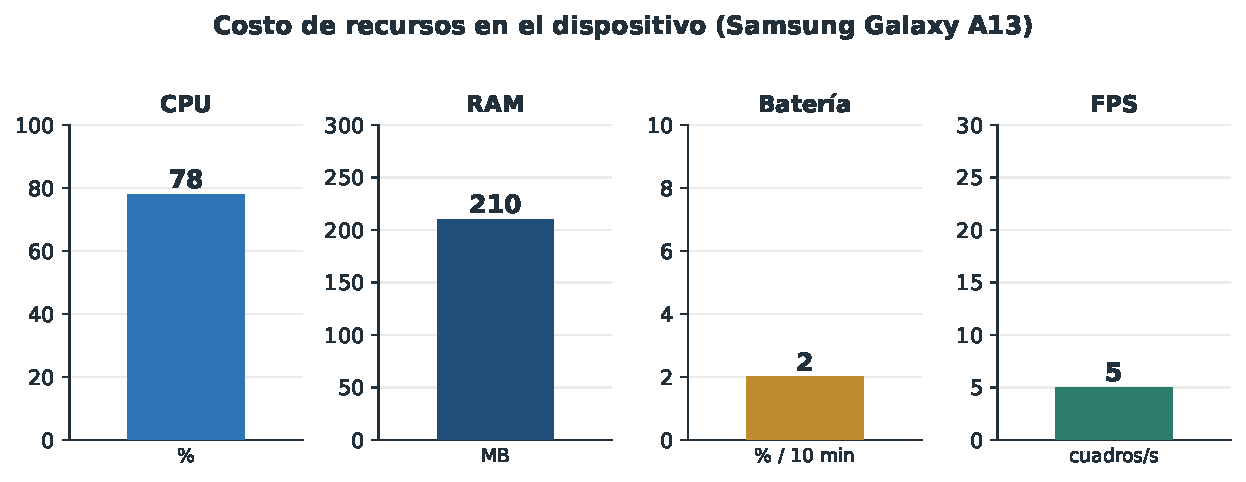
\includegraphics[width=0.85\linewidth]{Figures/Resultados/recursos_dispositivo.pdf}
    \caption[Costo de recursos en el dispositivo]{Costo de recursos del sistema en el Samsung Galaxy A13 durante el reconocimiento de una seña dinámica: uso de CPU, memoria, consumo de batería por cada diez minutos de uso continuo y cuadros por segundo procesados. Fuente: Elaboración propia.}
    \label{fig:recursos}
\end{figure}

El uso de CPU cercano al 78\% y los 210 MB de memoria son cargas altas para un teléfono de gama baja, coherentes con el procesamiento de dos manos y del cuerpo en cada fotograma. El consumo de batería, de alrededor del 2\% cada diez minutos de uso continuo, es moderado y compatible con las sesiones cortas y frecuentes que plantea el sistema.


\section{Instrumentos para la evaluación de usabilidad}

Esta sección presenta los dos instrumentos con que se medirá la percepción de las personas usuarias. Su aplicación con la Fundación CasAyuda queda pendiente al cierre de este documento, de modo que aquí se documenta su diseño y su justificación, no resultados. El \autoref{chap:conclusiones} retoma su aplicación como la primera tarea del trabajo que resta.

La percepción de las personas usuarias se evalúa con dos instrumentos, uno por cada tipo de participante, y de forma anónima. En ambos se registra la edad, el rol y el nivel de conocimiento del \Acrshort{lesho}, para interpretar los resultados en su contexto. La distinción es necesaria porque el público incluye tanto a personas adultas, que valoran la herramienta, como a niños sordos, cuyo perfil exige un instrumento accesible.

Para las personas adultas, como docentes, intérpretes, familiares y personal de la fundación, se emplea un cuestionario breve y de lenguaje sencillo. Se apoya en las dimensiones reconocidas de usabilidad, como la facilidad de uso, el aprendizaje y la satisfacción, y toma como referencia la Escala de Usabilidad del Sistema (\acrfull{sus}) \cite{brooke_sus_1996}. A diferencia de la versión clásica de esa escala, que alterna afirmaciones a favor y en contra, aquí todas las afirmaciones se redactan en el mismo sentido y con palabras simples: la respuesta más favorable es siempre el mayor acuerdo. La Tabla~\ref{tab:instrumento} presenta este instrumento.

\begin{table}[h!]
\centering
\begin{tabular}{cl}
\hline
\textbf{\#} & \textbf{Afirmación (escala de 1 a 5, donde 5 es la respuesta más favorable)} \\
\hline
1 & La aplicación fue fácil de usar. \\
2 & Aprendí a usarla rápidamente. \\
3 & Los botones y los textos se veían claros y grandes. \\
4 & Siempre supe qué estaba pasando en la pantalla. \\
5 & Me sentí seguro al usarla. \\
6 & Me gustó usar la aplicación. \\
7 & Usaría esta aplicación otra vez. \\
8 & El texto que apareció al hacer las señas fue correcto. \\
9 & Las señas que hizo el muñeco se entendieron bien. \\
10 & La aplicación sirve para comunicarse con un niño sordo. \\
\hline
\end{tabular}
\caption{Instrumento de usabilidad para las personas adultas. Todas las afirmaciones van en el mismo sentido: el mayor acuerdo, 5, es siempre la respuesta más favorable.}
\label{tab:instrumento}
\end{table}

Cada afirmación se responde en una escala de 1 a 5, donde 1 es total desacuerdo y 5 total acuerdo, y en todas el 5 es la respuesta más favorable. Las respuestas se resumen en un gráfico de barras apiladas por afirmación, que muestra la proporción de participantes en cada nivel de acuerdo, y en un índice de satisfacción global obtenido como el promedio de las respuestas llevado a una escala de 0 a 100.

Para los niños sordos, que tienen el \Acrshort{lesho} como primera lengua y todavía no leen español con fluidez, un cuestionario de frases no es apropiado. En su lugar se utiliza un instrumento visual de caritas, tomado del Fun Toolkit \cite{read_funtoolkit_2006}, un método validado para recoger la opinión de los niños en su interacción con la tecnología. El intérprete formula cada pregunta en \Acrshort{lesho} y el niño señala la carita que representa su respuesta, sobre la escala de cinco niveles de la Figura~\ref{fig:smileyometer}, que va de muy mal a muy bien.

\begin{figure}[htbp]
    \centering
    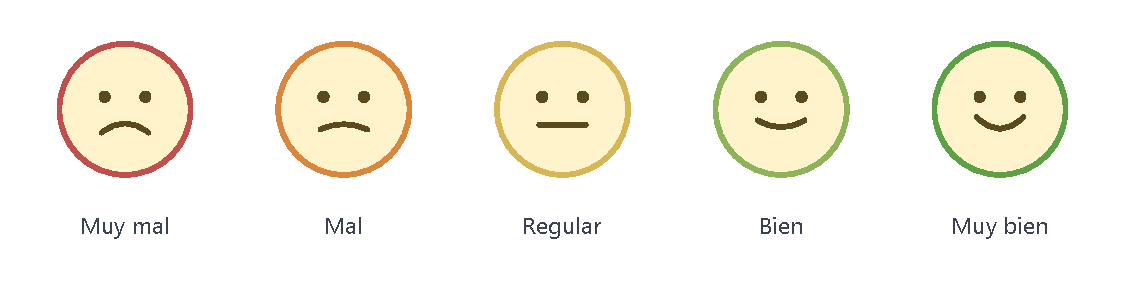
\includegraphics[width=0.85\linewidth]{Figures/Resultados/smileyometer.pdf}
    \caption[Escala de caritas para los niños]{Escala de caritas (\textit{Smileyometer}) con la que los niños señalan su respuesta, de muy mal a muy bien. Fuente: Elaboración propia, adaptada del Fun Toolkit.}
    \label{fig:smileyometer}
\end{figure}

Las preguntas dirigidas a los niños son cuatro, cortas y concretas:

\begin{itemize}
    \item ¿Te gustó la aplicación?
    \item ¿Entendiste las señas que hizo el muñeco?
    \item ¿Fue fácil de usar?
    \item ¿La usarías otra vez?
\end{itemize}

Cada respuesta se registra como una de las cinco caritas, y los resultados se resumen contando cuántos niños eligieron cada nivel en cada pregunta. La combinación de ambos instrumentos permite valorar tanto la usabilidad percibida por las personas adultas como la experiencia directa de los niños, que son los usuarios finales del sistema.


\section{Discusión integral de los resultados}

Los resultados permiten sostener que el sistema cumple su objetivo técnico central: reconocer, de forma on-device y sin conexión, tanto el alfabeto dactilológico como un vocabulario de señas dinámicas del \Acrshort{lesho}. El Modelo A alcanza una exactitud de 99.54\% y el Modelo B una de 98.80\%, ambos con modelos muy livianos que caben con holgura en un teléfono de gama baja.

El análisis por clase revela un patrón consistente y valioso para el diseño. Las señas que se distinguen por el lugar de articulación se reconocen con solidez, gracias a la incorporación de la ubicación de la mano y de la punta del índice en el vector de entrada. Las señas que comparten lugar y difieren solo en la forma o el movimiento de la mano son las más difíciles, y son las que más se benefician de contar con más datos y más personas.

Se identifican tres limitaciones honestas. Primero, aunque la evaluación se hizo sobre tomas que el modelo no vio, el conjunto de personas es todavía reducido, por lo que la generalización a una población más amplia debe confirmarse al ampliar el corpus. Segundo, las señas y letras que dependen del movimiento son más sensibles a la variación entre personas que las poses fijas. Tercero, en el dispositivo de gama baja la tasa de fotogramas por segundo es baja, lo que exige capturar la seña con cuidado y sostener la posición inicial; esta restricción de uso se documenta en el manual.

En conjunto, los resultados validan las decisiones metodológicas del proyecto y delimitan con claridad el trabajo que resta: seguir ampliando el corpus a más personas para reforzar la generalización, y aplicar los instrumentos de usabilidad ya diseñados con las personas usuarias de la fundación. Estos puntos se desarrollan en el capítulo de conclusiones y recomendaciones.
